%Capítulo 3

\chapter{Calibración clásica}
\label{ch:objetivo}
\lhead{\emph{Calibración clásica}}
%----------------------------------------------------------------------------------------

\section{Calibración clásica}

En la calibración interna se utilizan lazos de calibración, los cuales son utilizados para calibrar.

Como fue introducido previamente, una antena consta de un generador, una RFDN y el panel de módulos radiantes. Como puede
variar el comportamiento de cada componente, se utiliza la calibración. En particular, este método se lo utiliza para poder 
medir, detectar y corregir el mal funcionamiento de parte de la RFDN, en particular todas las desviaciones se las atribuyen 
los módulos de Transmisión/Recepción. A su vez, también se puede detectar si uno de dichos módulos queda inhabilitado a 
causa que cierta parte de la cadena de transmisión/recepción o dicho componente se destruyó.

Como limitación, esta calibración interna no puede medir las partes pasivas del sistema que están fuera del lazo de 
calibración interna (por ejemplo los módulos radiantes), ni la ganancia absoluta, debido a la ausencia de un target standard
de calibración \cite{Wang2010}. 


En la figura \ref{fig:classic_cal_scheme} se muestra el esquema de calibración, en el cual se observan tres modos de 
calibración. Cada uno posee distintos caminos, \textbf{P1} (líneas rojas) caracteriza el camino de transmisión, \textbf{P2}
(línea azul) caracteriza el camino de recepción y \textbf{P3} la electrónica central (CE) junto a los puertos auxiliares de 
transmisión/recepción. \textbf{P3} es utilizado para corregir posibles variaciones en los pulsos \textbf{P1} y \textbf{P2} 
\cite{Makhoul2012}

\begin{figure}[H]
 \centering
 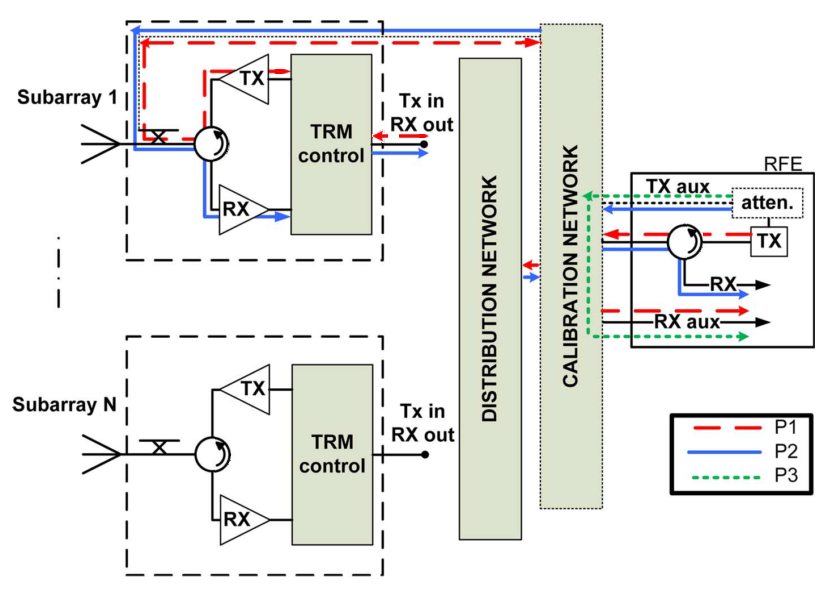
\includegraphics[width=10cm]{gfx/classic_cal_scheme.png}
 \caption{Esquema de calibración interna: camino de calibración de pulsos \textbf{P1} (Tx) en rojo, \textbf{P2} (Rx) en azul 
 y \textbf{P3} (electrónica central) en verde \cite{Makhoul2012}.}
 \label{fig:classic_cal_scheme}
\end{figure}

\subsection{Método}

A parte de la medición de la estabilidad del instrumento, es necesario obtener el funcionamiento de los TRMs de forma 
individual. Como el apuntamiento y la planitud de la señal dependen de la configuración de estos componentes, es necesario 
conocer su estado actual de funcionamiento. Comparando con datos de telemetría (ejemplo temperaturas y tensiones de los 
TRMs) junto a apropiada caracterización en tierra solo provee información limitada del comportamiento del radar \cite{Br2007}.

Una estrategia para mediciones individuales de cada TRM requiere que el resto esté apagado. El problema de esta estrategia 
es que, al tener parte de la antena apagada, no resulta un método representativo al modo de funcionamiento nominal (toda la 
antena operativa). Para solventar esta problemática y calibrar todos los TRMs a la vez, al menos en transmisión o recepción,
se hace uso de los defasadores para armar un código en que las señales sean ortogonales. En particular, por ejemplo, una de
las usos es defasar cada TRM en $\pm90^{\circ}$ siguiendo una determinada secuencia $c_{mn}(t)$ por cada uno.

\begin{figure}[!H]
 \centering
 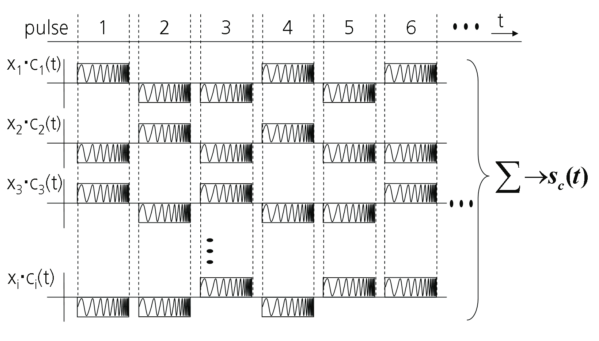
\includegraphics[width=8cm]{gfx/superposition_signals_classic.png}
 \caption{Superposición de señales de todos los TRMs. Cada señal tiene su propia secuencia de código aplicada entre pulsos \cite{Br2007}.}
 \label{fig:sup_sign_classic}
\end{figure}

Por lo tanto, la fase de salida de cada TRM es la fase configurada $\varphi_{mn}$ sumada al defasaje del código de 
$90^{\circ}$. Consecuentemente, la superposición de todas las ganancias de los TRMs, $a_{mn}$, y fases, $\varphi_{mn}$,
es obtenida en el puerto de recepción la la RFDN, $s_c(t)$ como se muestra en la figura \ref{fig:sup_sign_classic}.

\begin{equation}
	s_c(t) = \sum_{m=0}^{M-1}\sum_{n=0}^{N-1}c_{mn}\cdot a_{mn}e^{j\varphi{mn}} + n_{mn}
\end{equation}

Donde $n_{mn}$ es el ruido inherente que hay en las mediciones de cada TRM. Para decodificar y obtener la ganancia 
$\tilde{a}_{mn}$ y fase estimada $\tilde\varphi_{mn}$ de algún TRM, la señal compuesta $s_c$ es correlacionada con 
la secuencia del módulo deseado. Con esta correlación la modulación de la secuencia se elimina dando como resultado
la ganancia estimada.

\begin{equation}
\begin{aligned}
	\tilde{x}_{mn} &= s_c \otimes c^*_{mn} \\
	\tilde{x}_{mn} = \int s_c(t) &\cdot c^*_{mn}(t) dt = \tilde{a}_{mn}e^{j\tilde{\varphi}_{mn}} \\
\end{aligned}
\label{eq:}
\end{equation}

En general el código de calibración utilizado es el código walsh. Dicho código deriva de las matrices de Hadamard (ver 
apéndice \ref{AppendixB}); dada sus propiedades de ortonormalidad, cada código, o fila, es unívocamente distinguible del 
resto. Para minimizar la cantidad de mediciones, el largo del código ($l$) debe ser lo más corto positble. El número de 
TRMs de la antena es el determinante de la cota inferior.

\begin{equation}
	l = 2^i \ge N \cdot M
\end{equation}

Siendo $N$ la cantidad de filas y $M$ la cantidad de paneles, o columnas, que tiene el array de antena. No es necesario que 
se calibren todos los TRMs de una. Hay tres estrategias que se utilizan con este método de calibración para obtener 
distintos niveles de granularidad de mediciones a saber.

\begin{itemize}
	\item \textbf{Nivel módulo:} Este nivel es el que utiliza los códigos más largos, dado que se calibran todos los módulos que 
		posee la antena en una polarización determinada ($l = 2^i \ge N \cdot M$).
	\item \textbf{Nivel panel:} En este nivel se utiliza el mismo código para todos los TRMs que son de un mismo panel, 
		logrando así, decrecer el largo del código ($l = 2^i \ge M$).
	\item \textbf{Nivel fila:} En este nivel se utiliza el mismo código para todos los TRMs que son de una misma fila, 
		logrando así, decrecer el largo del código ($l = 2^i \ge N$).
\end{itemize}

Este método a nivel panel y fila sirve para la caracterización del la configuración del apuntamiento de antena \cite{Br2007}.



Para eliminar el error en la estimación de la ganancia del primer RM, es necesario que se evite la utilización de la 
primer columna de la matriz de Hadamard \cite{Wang2010}.

